\documentclass[border=10pt]{standalone}

\usepackage{tikz}
\usepackage{tikzsymbols}
\usetikzlibrary{calc,patterns,shapes.geometric}

\def\centerarc[#1](#2)(#3:#4:#5){\draw[#1] ($(#2)+({#5*cos(#3)},{#5*sin(#3)})$) arc (#3:#4:#5);}

\begin{document}
	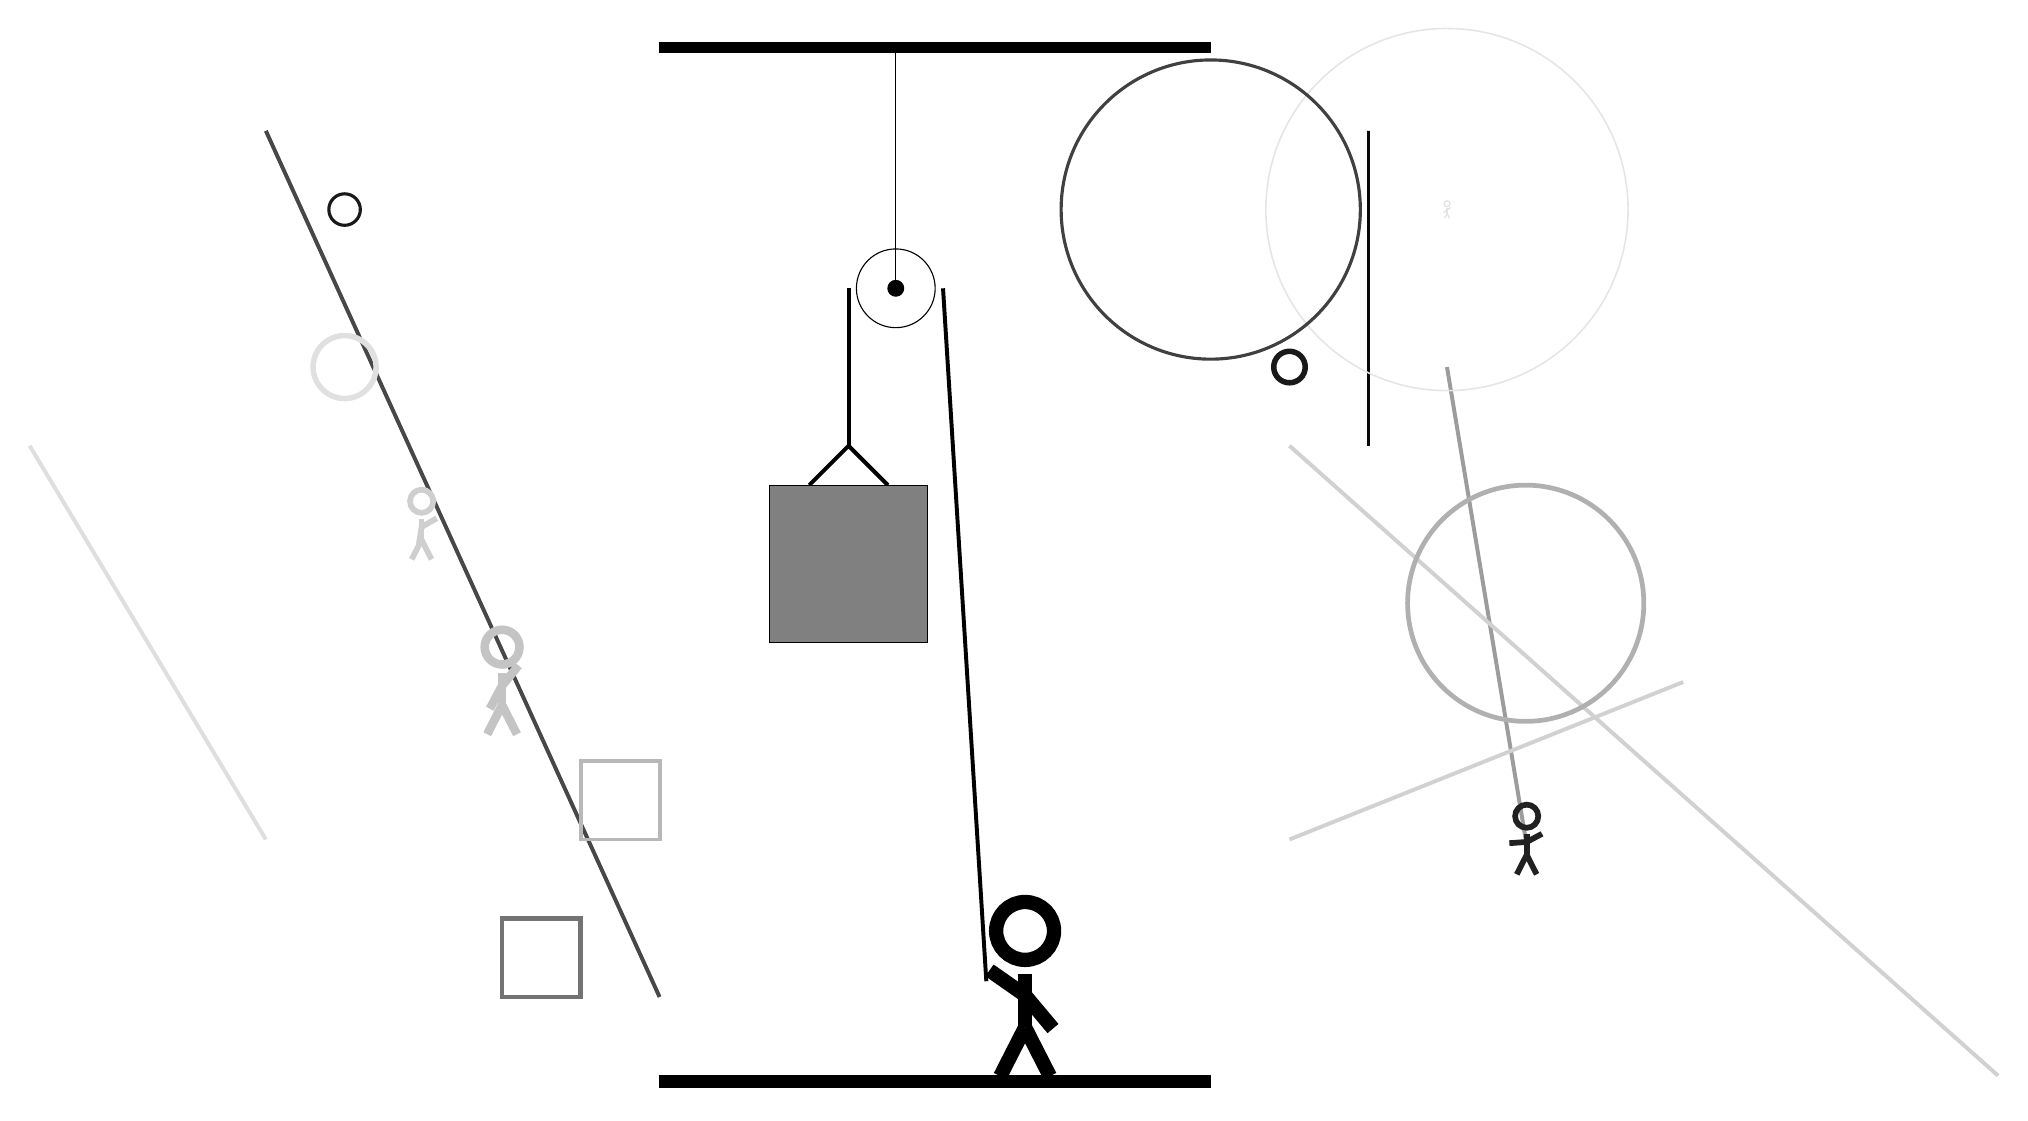
\begin{tikzpicture}
		%%%%% START %%%%%
		
		\draw[fill=black] (-2, 10) rectangle (5, 10.125);
		
		\draw (1, 7) circle (0.5);
		\draw[fill=black] (1, 7) circle (0.1);
		\draw (1, 10) -- (1, 7);
		
		\draw[line width=0.5mm] (-0.1, 4.5) -- (0.4, 5.0) -- (0.9, 4.5);
		\draw[fill=black!50] (-0.6, 4.5) rectangle (1.4, 2.5);
		
		\draw [line width=0.7mm, color=black!90](6, 6) circle (0.2);
		
		\draw [line width=0.4mm, color=black!90](-6, 8) circle (0.2);
		\draw[line width=0.4mm, color=black!97] (7, 5) rectangle (7, 9);
		\draw[line width=0.6mm, color=black!55] (-4, -2) rectangle (-3, -1);
		\draw[line width=0.5mm, color=black!39](9, 0) -- (8, 6);
		\draw[line width=0.5mm, color=black!18](6, 5) -- (15, -3);
		
		\draw [line width=0.6mm, color=black!31](9, 3) circle (1.5);
		\draw[line width=0.5mm, color=black!18](6, 0) -- (11, 2);
		\draw[line width=0.5mm, color=black!13](-7, 0) -- (-10, 5);
		\draw[line width=0.5mm, color=black!72](-2, -2) -- (-7, 9);
		\draw [line width=0.7mm, color=black!12](-6, 6) circle (0.4);
		\draw[line width=0.5mm, color=black!28] (-2, 0) rectangle (-3, 1);
		\node[line width=0.7mm, color=black!11] at (8, 8) {\Strichmaxerl[1][34][38]};
		
		\draw [line width=0.2mm, color=black!10](8, 8) circle (2.3);
		\draw [line width=0.4mm, color=black!75](5, 8) circle (1.9);
		\node[line width=0.4mm, color=black!19] at (-5, 4) {\Strichmaxerl[4][81][30]};
		\node[line width=0.6mm, color=black!23] at (-4, 2) {\Strichmaxerl[6][62][51]};
		\node[line width=0.6mm, color=black!87] at (9, 0) {\Strichmaxerl[4][4][28]};
		
		\draw[line width=0.5mm] (0.4, 7) -- (0.4, 5.0);
		\centerarc[line width=0.5mm](1, 7)(0:180:0.6);
		\draw[line width=0.5mm](1.6, 7) -- (2.15, -1.8);
		
		\node at (2.6, -1.9) {\Strichmaxerl[10][-35][-50]};
		
		\draw[fill=black] (-2, -3) rectangle (5, -3.15);
		
		%%%%% END %%%%%
	\end{tikzpicture}
\end{document}